% questions.tex —— 1989 年·全国卷·理科 · 题目内容片段（无答案）
% 由 tools/generate_projects.py 依来源总账自 1989/1989_数学真题_全国理_试题.md 生成，勿手改（改源 MD 后重跑）


\gkpart{试题}

\begin{gktip}
\textbf{来源说明}：固定源为一页 A3 三栏排印稿，印刷页码 34，含第 1—24 题及两幅图；没有答案、解析或分值。按该页逐题核对转录，补集、命题否定及复数共轭上的横线按源图保留。

\textbf{图形说明}：圆柱、平行六面体均用 TikZ 绘制，仅表达原图标号和题设关系，不从投影视角补充度量条件。
\end{gktip}

\begin{question}
\gkti{1}

如果 $I=\{a,b,c,d,e\}$，$M=\{a,c,d\}$，$N=\{b,d,e\}$，其中 $I$ 是全集，那么 $\overline M\cap\overline N$ 等于\mbox{（　　）}

（A）$\varnothing$　　（B）$\{d\}$　　（C）$\{a,c\}$　　（D）$\{b,e\}$

\end{question}
\begin{question}
\gkti{2}

与函数 $y=x$ 有相同图象的一个函数是\mbox{（　　）}

（A）$y=\sqrt{x^2}$　　（B）$y=\dfrac{x^2}{x}$

（C）$y=a^{\log_a x}$，其中 $a>0$，$a\ne1$

（D）$y=\log_a a^x$，其中 $a>0$，$a\ne1$

\end{question}
\begin{question}
\gkti{3}

如果圆锥的底面半径为 $\sqrt2$，高为 $2$，那么它的侧面积是\mbox{（　　）}

（A）$4\sqrt3\pi$　　（B）$2\sqrt2\pi$　　（C）$2\sqrt3\pi$　　（D）$4\sqrt2\pi$

\end{question}
\begin{question}
\gkti{4}

$\cos\left[\arcsin\left(-\dfrac45\right)-\arccos\left(-\dfrac35\right)\right]$ 的值等于\mbox{（　　）}

（A）$-1$　　（B）$-\dfrac7{25}$　　（C）$\dfrac7{25}$　　（D）$-\dfrac{\sqrt{10}}5$

\end{question}
\begin{question}
\gkti{5}

已知 $\{a_n\}$ 是等比数列，如果 $a_1+a_2+a_3=18$，$a_2+a_3+a_4=-9$，且 $S_n=a_1+a_2+\cdots+a_n$，那么 $\displaystyle\lim_{n\to\infty}S_n$ 的值等于\mbox{（　　）}

（A）$8$　　（B）$16$　　（C）$32$　　（D）$48$

\end{question}
\begin{question}
\gkti{6}

如果 $|\cos\theta|=\dfrac15$，$\dfrac52\pi<\theta<3\pi$，那么 $\sin\dfrac\theta2$ 的值等于\mbox{（　　）}

（A）$-\dfrac{\sqrt{10}}5$　　（B）$\dfrac{\sqrt{10}}5$　　（C）$-\dfrac{\sqrt{15}}5$　　（D）$\dfrac{\sqrt{15}}5$

\end{question}
\begin{question}
\gkti{7}

设复数 $z$ 满足关系式 $z+|\overline z|=2+i$，那么 $z$ 等于\mbox{（　　）}

（A）$-\dfrac34+i$　　（B）$\dfrac34-i$　　（C）$-\dfrac34-i$　　（D）$\dfrac34+i$

\end{question}
\begin{question}
\gkti{8}

已知球的两个平行截面的面积分别为 $5\pi$ 和 $8\pi$，它们位于球心的同一侧，且相距为 $1$，那么这个球的半径是\mbox{（　　）}

（A）$4$　　（B）$3$　　（C）$2$　　（D）$5$

\end{question}
\begin{question}
\gkti{9}

已知椭圆的极坐标方程是 $\rho=\dfrac5{3-2\cos\theta}$，那么它的短轴长是\mbox{（　　）}

（A）$\dfrac{10}3$　　（B）$\sqrt5$　　（C）$2\sqrt5$　　（D）$2\sqrt3$

\end{question}
\begin{question}
\gkti{10}

如果双曲线 $\dfrac{x^2}{64}-\dfrac{y^2}{36}=1$ 上一点 $P$ 到它的右焦点的距离是 $8$，那么点 $P$ 到它的右准线的距离是\mbox{（　　）}

（A）$10$　　（B）$\dfrac{32\sqrt7}{7}$　　（C）$2\sqrt7$　　（D）$\dfrac{32}{5}$

\end{question}
\begin{question}
\gkti{11}

已知 $f(x)=8+2x-x^2$，如果 $g(x)=f(2-x^2)$，那么 $g(x)$\mbox{（　　）}

（A）在区间 $(-1,0)$ 上是减函数　　（B）在区间 $(0,1)$ 上是减函数

（C）在区间 $(-2,0)$ 上是增函数　　（D）在区间 $(0,2)$ 上是增函数

\end{question}
\begin{question}
\gkti{12}

由数字 $1,2,3,4,5$ 组成没有重复数字的五位数，其中小于 $50000$ 的偶数共有\mbox{（　　）}

（A）$60$ 个　　（B）$48$ 个　　（C）$36$ 个　　（D）$24$ 个

\end{question}
\begin{question}
\gkti{13}

方程 $\sin x-\sqrt3\cos x=\sqrt2$ 的解集是 $\underline{\hspace{8em}}$。

\end{question}
\begin{question}
\gkti{14}

不等式 $|x^2-3x|>4$ 的解集是 $\underline{\hspace{7em}}$。

\end{question}
\begin{question}
\gkti{15}

函数 $y=\dfrac{e^x-1}{e^x+1}$ 的反函数的定义域是 $\underline{\hspace{6em}}$。

\end{question}
\begin{question}
\gkti{16}

已知 $(1-2x)^7=a_0+a_1x+a_2x^2+\cdots+a_7x^7$，那么 $a_1+a_2+\cdots+a_7=\underline{\hspace{5em}}$。

\end{question}
\begin{question}
\gkti{17}

已知 $A$ 和 $B$ 是两个命题，如果 $A$ 是 $B$ 的充分条件，那么 $B$ 是 $A$ 的 $\underline{\hspace{4em}}$ 条件；$\overline A$ 是 $\overline B$ 的 $\underline{\hspace{4em}}$ 条件。

\Needspace{0.4\textheight}
\end{question}
\begin{question}
\gkti{18}

如图，已知圆柱的底面半径是 $3$，高是 $4$，$A$、$B$ 两点分别在两底面的圆周上，并且 $AB=5$，那么直线 $AB$ 与轴 $OO'$ 之间的距离等于 $\underline{\hspace{5em}}$。
\nopagebreak[4]
\begin{center}% 固定源印刷页34：圆柱两底面圆周上的A/B和轴OO'；投影不量角。
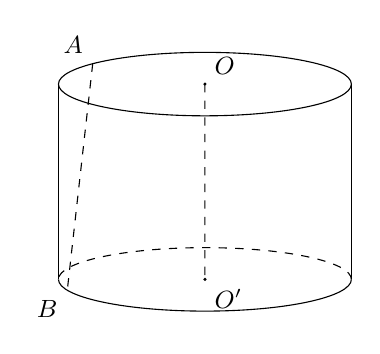
\begin{tikzpicture}[scale=0.62,font=\small]
  \coordinate (O) at (0,4);
  \coordinate (Oprime) at (0,0);
  \coordinate (A) at ({3*cos(140)},{4+0.65*sin(140)});
  \coordinate (B) at ({3*cos(200)},{0.65*sin(200)});
  \draw (O) ellipse[x radius=3,y radius=0.65];
  \draw (-3,4)--(-3,0) (3,4)--(3,0);
  \draw (3,0) arc[start angle=0,end angle=-180,x radius=3,y radius=0.65];
  \draw[dashed] (3,0) arc[start angle=0,end angle=180,x radius=3,y radius=0.65];
  \draw[dashed] (O)--(Oprime) (A)--(B);
  \fill (O) circle (1pt) node[above right] {$O$};
  \fill (Oprime) circle (1pt) node[below right] {$O'$};
  \node[above left] at (A) {$A$};
  \node[below left] at (B) {$B$};
\end{tikzpicture}
\end{center}
\nopagebreak[4]
\end{question}
\begin{question}
\gkti{19}

\Needspace{5\baselineskip}
证明：

\nopagebreak[4]
\[
\tan\frac{3x}{2}-\tan\frac{x}{2}=\frac{2\sin x}{\cos x+\cos2x}\text{。}
\]

\Needspace{0.4\textheight}
\end{question}
\begin{question}
\gkti{20}

如图，在平行六面体 $ABCD-A_1B_1C_1D_1$ 中，已知 $AB=5$，$AD=4$，$AA_1=3$，$AB\perp AD$，$\angle A_1AB=\angle A_1AD=\dfrac\pi3$。

（1） 求证：顶点 $A_1$ 在底面 $ABCD$ 的射影 $O$ 在 $\angle BAD$ 的平分线上；

（2） 求这个平行六面体的体积。
\nopagebreak[4]
\begin{center}% 固定源印刷页34；与全国文第21题相同题设的斜棱平行六面体及射影。
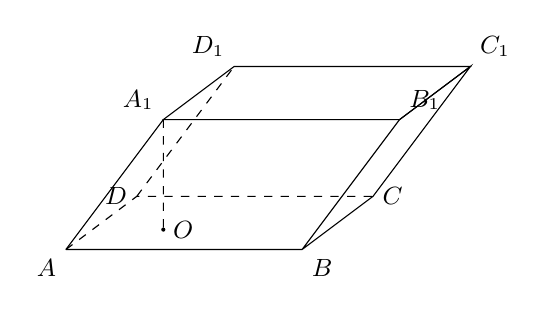
\begin{tikzpicture}[scale=0.75,font=\small]
  \coordinate (A) at (0,0);
  \coordinate (B) at (4,0);
  \coordinate (D) at (1.2,0.9);
  \coordinate (C) at (5.2,0.9);
  \coordinate (A1) at (1.65,2.2);
  \coordinate (B1) at (5.65,2.2);
  \coordinate (D1) at (2.85,3.1);
  \coordinate (C1) at (6.85,3.1);
  \coordinate (O) at (1.65,0.3375);
  \draw (A)--(B)--(C)--(C1)--(B1)--(B) (A)--(A1);
  \draw (A1)--(B1)--(C1)--(D1)--cycle;
  \draw[dashed] (A)--(D)--(C) (D)--(D1) (A1)--(O);
  \fill (O) circle (1pt) node[right] {$O$};
  \node[below left] at (A) {$A$};
  \node[below right] at (B) {$B$};
  \node[right] at (C) {$C$};
  \node[left] at (D) {$D$};
  \node[above left] at (A1) {$A_1$};
  \node[above right] at (B1) {$B_1$};
  \node[above right] at (C1) {$C_1$};
  \node[above left] at (D1) {$D_1$};
\end{tikzpicture}
\end{center}
\nopagebreak[4]
\end{question}
\begin{question}
\gkti{21}

自点 $A(-3,3)$ 发出的光线 $L$ 射到 $x$ 轴上，被 $x$ 轴反射，其反射光线所在直线与圆 $x^2+y^2-4x-4y+7=0$ 相切，求光线 $L$ 所在直线的方程。

\end{question}
\begin{question}
\gkti{22}

已知 $a>0$，$a\ne1$，试求使方程 $\log_a(x-ak)=\log_{a^2}(x^2-a^2)$ 有解的 $k$ 的取值范围。

\end{question}
\begin{question}
\gkti{23}是否存在常数 $a,b,c$ 使得等式

\nopagebreak[4]
\[
1\cdot2^2+2\cdot3^2+\cdots+n(n+1)^2
=\frac{n(n+1)}{12}(an^2+bn+c)
\]

对一切自然数 $n$ 都成立？并证明你的结论。

\end{question}
\begin{question}
\gkti{24}

设 $f(x)$ 是定义在区间 $(-\infty,+\infty)$ 上以 $2$ 为周期的函数，对 $k\in\mathbb Z$，用 $I_k$ 表示区间 $(2k-1,2k+1]$，已知当 $x\in I_0$ 时，$f(x)=x^2$。

（1） 求 $f(x)$ 在 $I_k$ 上的解析表达式；

（2） 对自然数 $k$，求集合 $M_k=\{a\mid \text{\text{使方程} }f(x)=ax\text{ \text{在} }I_k\text{ \text{上有两个不等的实根}}\}$。

\end{question}